\begin{table}[htbp]
\centering
\caption{Mediciones de voltaje ánodo-cátodo $V_{AK}$ y corriente en el diodo para distintos LED. La columna $\pm$ corresponde a la incertidumbre de $V_{AK}$.}
\label{tab:mediciones_leds}

\scriptsize
\resizebox{\columnwidth}{!}{%
\begin{tabular}{lccccc}
\toprule
Color & $\lambda$ (\si{\nano\meter}) & $\nu$ (\si{\tera\hertz}) & $V_{AK}$ (\si{\volt}) & $\pm$ (\si{\volt}) & $I_{\mathrm{diodo}}$ \\
\midrule
Infrarrojo    & 940 & 318.928 & 0.89 & 0.01712 & $<\SI{0.1}{\micro\ampere}$ \\
Rojo          & 635 & 472.114 & 1.47 & 0.02176 & $<\SI{0.1}{\micro\ampere}$ \\
Naranja       & 595 & 503.853 & 1.46 & 0.02168 & $<\SI{0.1}{\micro\ampere}$ \\
Amarillo      & 585 & 512.466 & 1.61 & 0.02288 & $<\SI{0.1}{\micro\ampere}$ \\
Verde         & 525 & 571.033 & 1.89 & 0.02512 & $<\SI{0.1}{\micro\ampere}$ \\
Azul          & 465 & 644.715 & 2.14 & 0.02712 & $<\SI{0.1}{\micro\ampere}$ \\
Violeta       & 400 & 749.481 & 2.65 & 0.03120 & $\SI{6.0}{\micro\ampere}$ \\
Ultravioleta  & 390 & 768.699 & 2.66 & 0.03128 & $\SI{6.0}{\micro\ampere}$ \\
\bottomrule
\end{tabular}%
}
\end{table}

\begin{figure*}
    \centering
    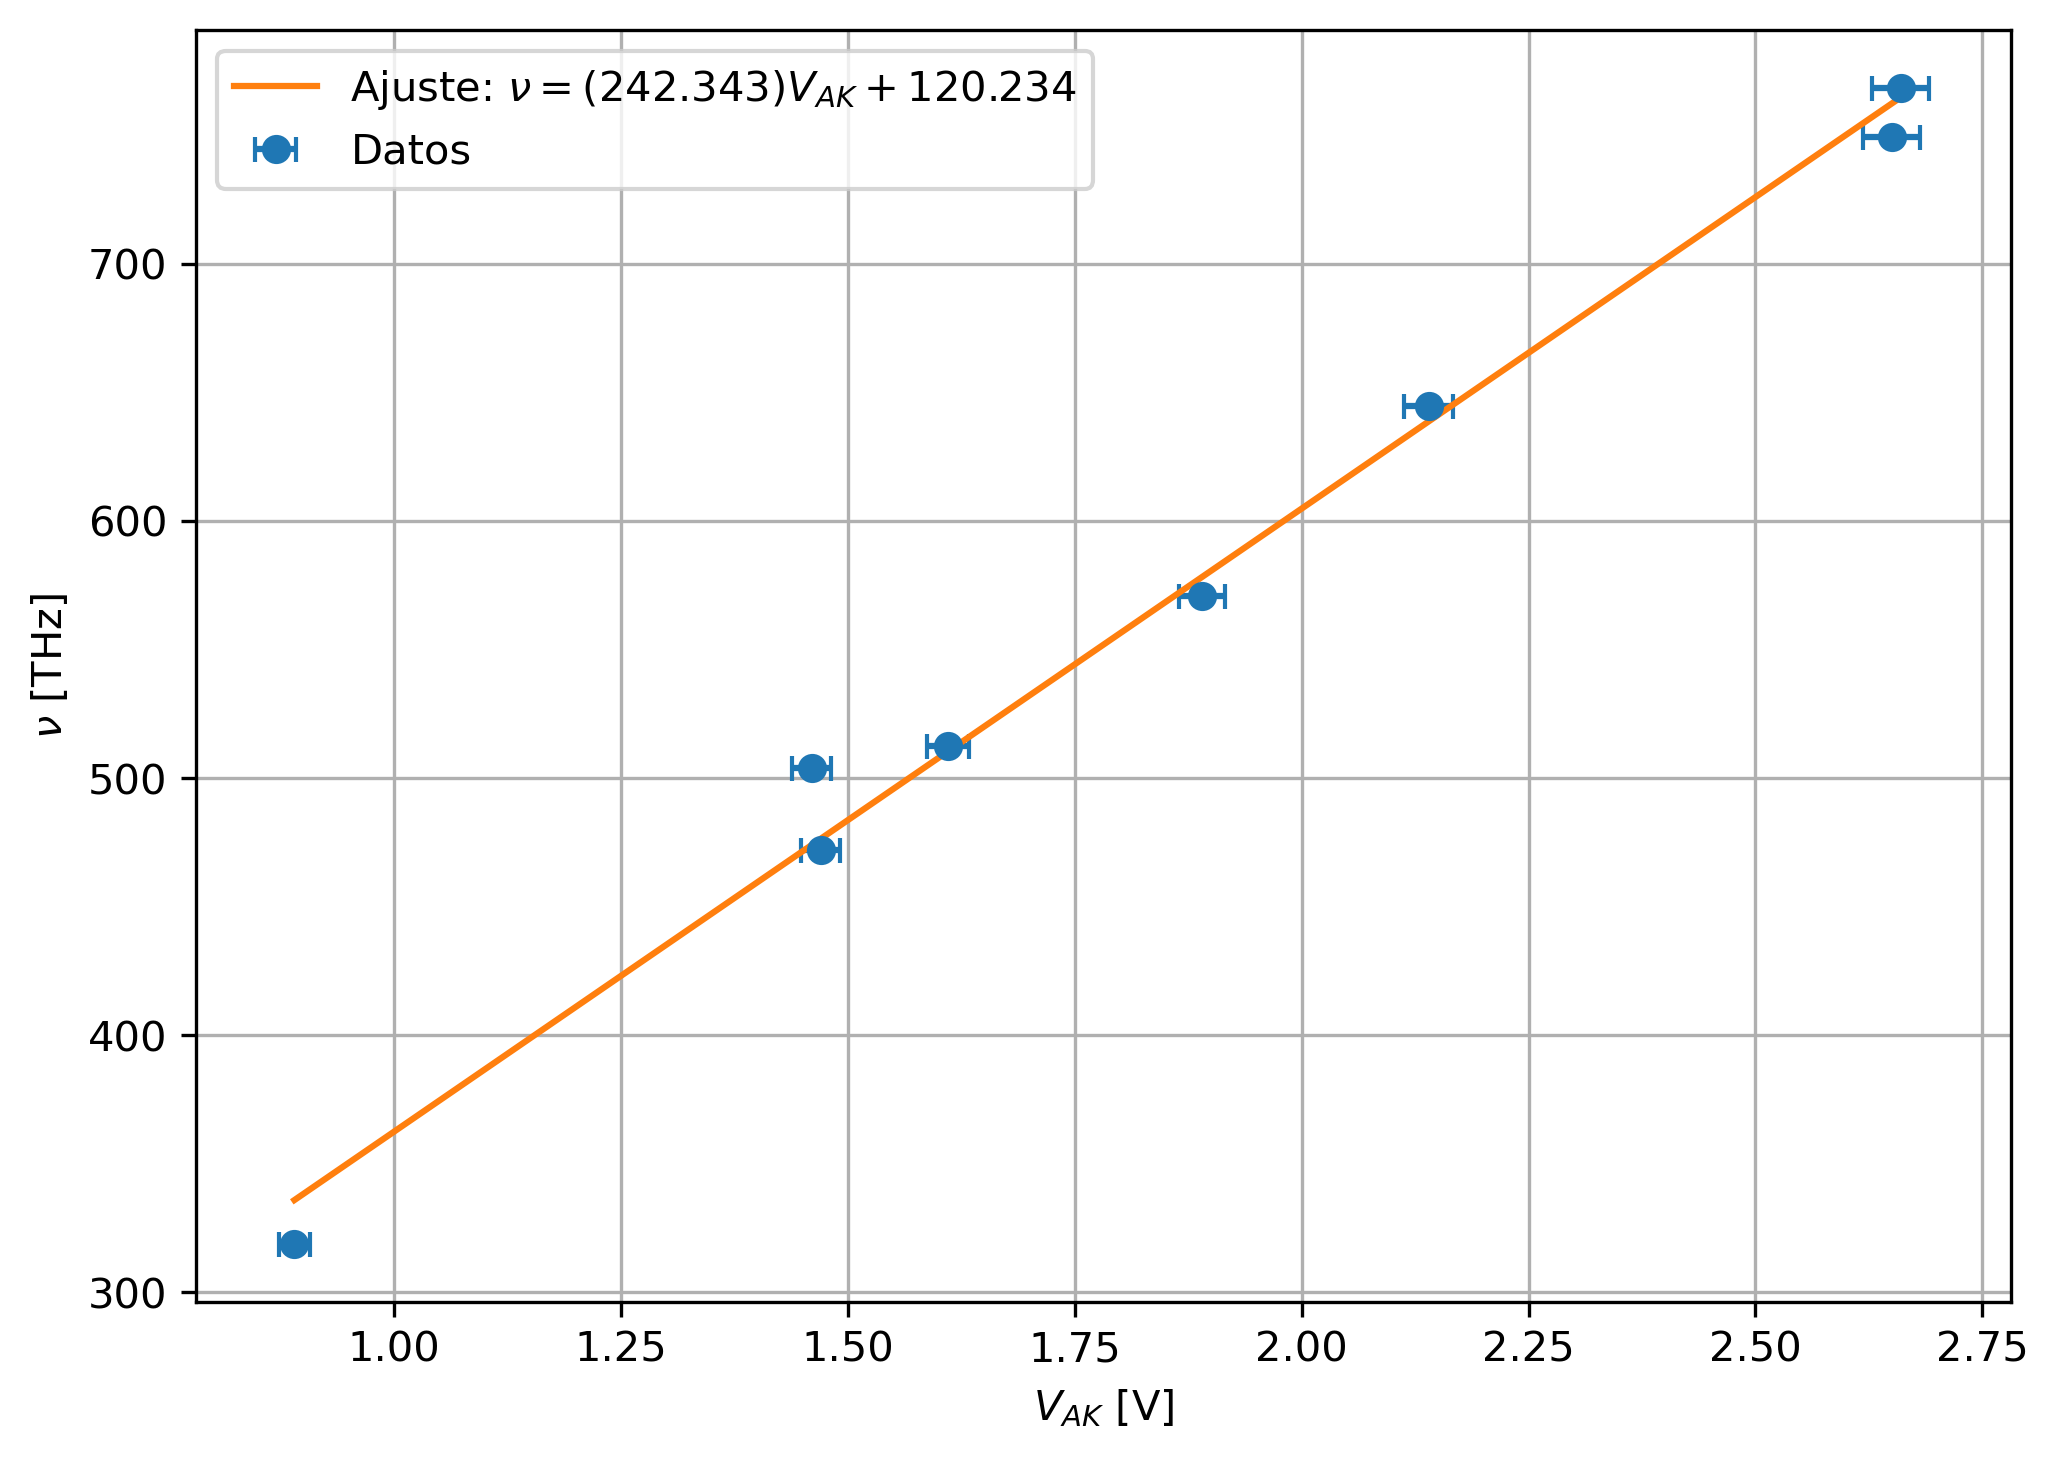
\includegraphics[width=0.7\linewidth]{figuras/graf_colores.png}
    \label{colores_graf}
    \captionof{figure}{Frecuencia $\nu$ contra voltaje $V_{A-K}$ y el ajuste lineal. En esta grafica los datos se invierten ya que el ajuste se realizo }
\end{figure*}


\begin{table}[htbp]
\centering
\caption{Resultados del ajuste lineal para la determinación de $h/e$.}
\label{tab:ajuste_he}

\scriptsize
\resizebox{\columnwidth}{!}{%
\begin{tabular}{lc}
\toprule
Magnitud & Valor \\
\midrule

$m$ &
$\left(
\SI{242.3}{} \pm \SI{9.6}{}
\right)\,\si{\tera\hertz\per\volt}$ \\

$b$ &
$\left(
\SI{120}{} \pm \SI{19}{}
\right)\,\si{\tera\hertz}$ \\

$R^2$ &
$\num{0.9907}$ \\

$\left(h/e\right)_{\mathrm{exp}}$ &
$\left(
\SI{4.13e-15}{} \pm \SI{0.16e-15}{}
\right)\,\si{\volt\second}$ \\

$\left(h/e\right)_{\mathrm{aceptado}}$ &
$\SI{4.135668e-15}{\volt\second}$ \\

$E_{\%}$ &
$\SI{-0.22}{\percent}$ \\

\bottomrule
\end{tabular}%
}
\end{table}

\begin{table}[htbp]
    \centering
    \caption{Longitud de onda correspondiente al máximo de intensidad
    y ancho espectral de los LED estudiados.}
    \label{tab:longitudes_onda_led}
    \small
    \setlength{\tabcolsep}{4pt}
    \begin{tabular}{lcc}
        \toprule
        LED
        & $\lambda_{\max}$ (\si{\nano\meter})
        & $\Delta\lambda$ (\si{\nano\meter}) \\
        \midrule
        Infrarrojo & 591.5 &  6.0  \\
        Rojo       & 631.6 &  6.2  \\
        Naranja    & 613.0 &  5.4  \\
        Amarillo   & 591.1 &  6.8  \\
        Verde      & 527.4 &  12.4 \\
        Azul       & 467.8 &  9.6  \\
        Violeta    & 399.5 &  6.3  \\
        Ultravioleta & 399.5 & 6.2 \\
        \bottomrule
    \end{tabular}
\end{table}
\newpage